\documentclass[journal]{IEEEtran}
\IEEEoverridecommandlockouts
\usepackage{cite}
\usepackage{amsmath,amssymb,amsfonts}
\usepackage{algorithmic}
\usepackage{algorithm}
\usepackage{array}
\usepackage{graphicx}
\usepackage{textcomp}
\usepackage{xcolor}
\usepackage{url}
\usepackage{orcidlink}
\usepackage{tikz}
\usepackage{float}
\usepackage{booktabs}
\usepackage{needspace}
\usepackage{capt-of}
\usepackage{etoolbox}

\makeatletter
\def\@IEEEBIOskipN{1.5\baselineskip}
\expandafter\patchcmd\csname\string\IEEEbiography\endcsname
  {\vskip \@IEEEBIOskipN plus 1fil minus 0\baselineskip}
  {\vskip \@IEEEBIOskipN}
  {}{\PackageWarning{main}{Unable to compact IEEE biography spacing}}
\makeatother


\def\BibTeX{{\rm B\kern-.05em{\sc i\kern-.025em b}\kern-.08em
    T\kern-.1667em\lower.7ex\hbox{E}\kern-.125emX}}
\begin{document}

\title{TWAPPA-FRL: Trust-Weighted Privacy-Preserving Aggregation for Federated Reinforcement Learning
in Collaborative Intrusion Detection}

\author{Piyumi M. S. Rajapaksha\textsuperscript{$\dagger$}~\orcidlink{0009-0002-6583-2652}, 
Artur Iasenovets\textsuperscript{$\dagger$}~\orcidlink{0009-0008-0008-3746}, 
Yinxue Yi~\orcidlink{0000-0003-4680-3389},
Fei Tang~\orcidlink{0000-0002-0048-9876}

\thanks{\textsuperscript{$\dagger$} The first two authors contributed equally to this paper.\\
Received Month Day, Year; revised Month Day, Year. This work was supported in 
part by the National Key Research and Development Program of China under Grant 2021YFF0704102, 
in part by the Key Project of Science and Technology Research by Chongqing Education Commission 
under Grant KJZD-K202400610, in part by the Chongqing Natural Science Foundation General 
Project under Grant CSTB2025NSCQ-GPX1263, and in part by the Youth Project of Science and 
Technology Research Program of Chongqing Municipal Education Commission of China under Grant KJQN202600608.
(\emph{Corresponding authors: Yinxue Yi, Fei Tang.})

Piyumi M. S. Rajapaksha and Yinxue Yi are with the School of Cybersecurity and Information Law, 
Chongqing University of Posts and Telecommunications, Chongqing 400065, China 
(email:  l201930026@stu.cqupt.edu.cn, yiyinxue@cqupt.edu.cn).
Artur Iasenovets and Fei Tang are with the School of Cybersecurity and Information Law, 
Chongqing University of Posts and Telecommunications, Chongqing 400065, China 
(email: L202420002@stu.cqupt.edu.cn, tangfei@cqupt.edu.cn).
}}

\maketitle

\begin{abstract}
Federated reinforcement learning (FRL) enables distributed intrusion-detection
agents to collaboratively improve a shared traffic-classification policy without
exchanging raw traffic data. However, model updates can still reveal sensitive
information about local environments, while conventional uniform aggregation gives
unreliable or adversarial clients the same influence as benign participants.
This paper presents TWAPPA-FRL, a secure and dependable FRL aggregation framework
for collaborative intrusion detection that composes Trust-Weighted Aggregation
(TWA), which suppresses unreliable or adversarial contributions, with
Privacy-Preserving Aggregation (PPA), which protects individual model updates during
aggregation. We evaluate the framework on a non-i.i.d. five-client CIC-IDS2017
setting with four benign and one malicious client under six individual poisoning
attacks, together with a federation-sensitivity study spanning five to twenty
clients. Across three fixed seeds, the TWA-enabled paths achieve mean round-30
accuracy of $0.9681$--$0.9737$ and macro-F1 of $0.9675$--$0.9734$. At the
predefined cutoff, the suppressed-round fraction is $100\%$ with one
malicious client among five and $86.7\%$ with one among ten; as malicious
participation increases, TWA shifts from threshold-level suppression to influence
attenuation. TWA--PPA matches plaintext TWA utility, requires $9.807$~s per round,
and uploads $2.745$~MiB per client and $13.723$~MiB system-wide per round.
These results demonstrate the feasibility of combining trust-weighted adversarial
suppression with HE-based privacy-preserving aggregation within a unified FRL
framework for collaborative intrusion detection, while identifying communication
efficiency, deployment scalability, verifiable trust computation, and decentralized
key management as priorities for future work.
\end{abstract}

\begin{IEEEkeywords}
Federated reinforcement learning, intrusion detection,
trust-aware aggregation, privacy-preserving aggregation,
homomorphic encryption
\end{IEEEkeywords}

\section{INTRODUCTION}\label{sec:introduction}

\subsection{Motivation and Problem Statement}
\IEEEPARstart{I}{ntelligent} intrusion detection increasingly requires distributed
learning across heterogeneous organizations, edge nodes, and monitoring
domains~\cite{mcmahan2017fedavg,kairouz2021flsurvey, srimali2026ica3pp}.
Network traffic is non-stationary, imbalanced, and sensitive, requiring systems
to both detect threats and select appropriate responses. Centralized intrusion
detection relies on collecting raw traffic at a single location, creating
privacy, confidentiality, and deployment challenges in multi-domain settings.

Federated learning (FL) partially addresses this problem by enabling multiple
participants to train a shared model without exchanging raw local
data~\cite{mcmahan2017fedavg,kairouz2021flsurvey}. This is useful for distributed
intrusion detection and network-defense
learning~\cite{chen2022feddef,chen2024ffids,manh2024homomorphic}. However,
conventional FL is usually formulated as supervised learning: clients upload
model updates, and a coordinator aggregates them using a rule such as FedAvg.
This does not fully capture the sequential decision-making nature of network
defense, where a system must learn policies that trade off detection utility,
operational disruption, and long-term reward.

Federated reinforcement learning (FRL) extends FL to this sequential setting.
Instead of merely learning a classifier, each client agent interacts with a
local environment, observes network states, classifies traffic, receives
rewards, and periodically contributes policy updates to a shared global model
\cite{chen2024reviewpfrl,li2024frlrl,yang2024fedprl,jing2025fmarlsurvey}.
Recent FRL and RL-assisted federated security systems apply this idea to
intrusion detection, malware mitigation, and adaptive response
\cite{vadigi2023frlids,feng2025cyberforce,kaur2025drrlflids}.
This makes FRL a natural fit for intrusion-detection and network-defense tasks 
such as traffic classification and adaptive intrusion response.

FRL-based intrusion detection, however, inherits two major limitations from
FL-based intrusion detection. First, raw model updates may reveal information about
local traffic distributions, attack prevalence, and training behavior even when
raw data remain local, creating leakage risks for local security conditions
\cite{chen2022feddef,chen2024ffids,hua2026privacy}. Second, FedAvg-style
aggregation does not distinguish reliable clients from poisoned or compromised
ones, a known vulnerability in FL-based NIDS settings
\cite{nguyen2020poisoningflnids,zhang2022secfednids,sun2024fedmade}, and can lead
to global model degradation. These limitations motivate the following research question:

\emph{How can we construct a federated reinforcement learning framework for collaborative
intrusion detection that supports both confidential model-update aggregation and trust-weighted
suppression of unreliable or adversarial clients?}

\subsection{Related Work}\label{sec:related_work}

To address the research question, we now review prior work along two dimensions:
privacy-preserving federated aggregation and robust/trust-aware federated aggregation.
A detailed comparison with representative systems is provided in
Table~\ref{tab:comparison-related} in Section~\ref{sec:experiments}.

1) \noindent\textbf{Privacy-Preserving Federated Aggregation:}

Bonawitz et al.~\cite{bonawitz2017secagg} introduce a masking-based secure
aggregation protocol for federated learning that lets a server recover only the
aggregate of high-dimensional client updates. 

BatchCrypt~\cite{zhang2020batchcrypt} proposes an HE-based cross-silo FL
system that reduces the cost of encrypted gradient aggregation by quantizing
gradients, batch-encoding them into long integers, and encrypting each batch
with additively homomorphic encryption. 

Manh et al.~\cite{manh2024homomorphic} propose a CKKS-enabled FL framework for
privacy-preserving intrusion detection in resource-constrained IoV networks,
using encrypted data offloading and encrypted FedAvg-style model aggregation.

Hercules~\cite{xuhercules2023} extends the POSEIDON-style $N$-party
privacy-preserving federated neural-network training setting with optimized
multiparty CKKS computation. 

2) \noindent\textbf{Robust and Trust-Aware Federated Aggregation:}

FLTrust~\cite{cao2021fltrust} proposes a trust-bootstrapped robust FL
aggregation method against poisoning attacks. It uses a small clean root dataset
at the server to derive a reference update, assigns ReLU-clipped cosine trust
scores to client updates, normalizes their magnitudes, and performs
trust-weighted averaging. 

FoolsGold~\cite{fung_limitations_2020} proposes a server-side robust FL
aggregation defense against sybil-based targeted poisoning. It assigns
per-client learning-rate weights using cosine similarity over historical client
updates, downweighting clients whose contributions appear unusually similar.

FLDetector~\cite{zhang_fldetector_2022} proposes a malicious-client filtering
defense for FL model-poisoning attacks. It predicts client updates from
historical update consistency and removes clients whose received updates deviate
from the predicted ones. 

FLAME~\cite{nguyen_flame_2022} proposes a robust FL defense framework for
mitigating backdoor attacks while preserving benign model utility. It combines
HDBSCAN-based model filtering, adaptive clipping, and Gaussian noising to remove
high-impact poisoned updates and neutralize remaining backdoor effects. 

3) \noindent\textbf{Joint Privacy and Robustness:}

Marx et al.~\cite{marx2026wwfl} propose WW-FL, an MPC-based hierarchical FL
framework in which clients secret-share training data to local MPC clusters and
global aggregation is performed over secret-shared cluster models, keeping the
global model private. 

Pillutla et al.~\cite{pillutla_robust_2022} propose a robust FL aggregation framework
(RFA) that replaces FedAvg's weighted arithmetic mean with an approximate geometric
median of client updates and preserves compatibility with secure-aggregation-style
MPC while improving robustness to data and update corruption. 

\textbf{Targeted gap.}
Privacy-preserving FL protects model updates but generally lacks
trust-weighted adversarial suppression
\cite{bonawitz2017secagg,zhang2020batchcrypt,manh2024homomorphic,
savposeidon2021,xuhercules2023}, whereas robust aggregation suppresses malicious
updates without confidential encrypted aggregation
\cite{cao2021fltrust,fung_limitations_2020,zhang_fldetector_2022,
nguyen_flame_2022}. RFA~\cite{pillutla_robust_2022} and
WW-FL~\cite{marx2026wwfl} partially bridge this gap in conventional FL, but
not in FRL-based intrusion detection. We combine both properties and evaluate them
in a non-i.i.d. federated intrusion-detection setting.

\subsection{Contributions}
We propose TWAPPA-FRL, a Trust-Weighted Privacy-Preserving Aggregation
framework for Federated Reinforcement Learning in Collaborative Intrusion
Detection. Its path-dependent design is detailed in
Section~\ref{sec:workflow_details}. The first core mechanism is trust-weighted
aggregation (TWA), described in Section~\ref{sec:trust_weighting}; the second is
privacy-preserving aggregation (PPA), described in
Section~\ref{sec:ppa_aggregation}. In the main TWA--PPA path, the two mechanisms
compose sequentially: TWA governs \emph{who influences} the global model and by how
much through trust-derived weights, whereas PPA limits \emph{who can observe}
individual update values during aggregation under the key-separation
assumptions and leakage model of Section~\ref{sec:security}.

The main contributions of this work are as follows:


\begin{enumerate}
  \item \textbf{Secure and dependable FRL framework for collaborative intrusion detection.}
  We define six controlled execution paths that isolate weighting and transport
  choices. Only the main TWA--PPA path composes trust-dependent influence control
  with encrypted aggregation; the others provide comparison variants.

  \item \textbf{Trust-dependent adversarial influence control.}
  TWA combines six components derived from rewards, updates, trust history, and local
  quality to determine aggregation influence, downweighting contributions assigned low
  trust without access to malicious labels.

  \item \textbf{CKKS-based confidential aggregation for FRL updates.}
  We implement PPA across three encrypted paths using contiguous packing of
  real-valued DQN updates, ciphertext-domain weighted summation, and
  aggregate-only decryption by a separate non-training key authority.

  \item \textbf{Path-dependent confidentiality and leakage analysis.}
  We specify threats, leakage, and exclusions and reduce ciphertext
  confidentiality against the honest-but-curious coordinator to CKKS IND-CPA/RLWE
  security under key separation and no coordinator--key-authority collusion. The
  analysis does not establish client-generated trust-metadata integrity.

  \item \textbf{Reproducible multi-seed evaluation and open-source release.}
  Across three fixed seeds, we evaluate all six paths under the clean condition and six
  standalone attack conditions and study federation sensitivity from five to
  twenty clients. We release the reproducibility materials at
  \url{https://github.com/hetiantian10/TWAPPA-FRL} and at 
  \url{https://doi.org/10.5281/zenodo.21872240}.
\end{enumerate}

\subsection{Organization}

The remainder of this paper is organized as follows.
Section~\ref{sec:preliminaries} introduces the preliminaries and notation.
Section~\ref{sec:proposed_system} presents the system model, threat model, and
execution workflow. Sections~\ref{sec:trust_weighting} and
\ref{sec:ppa_aggregation} describe TWA and PPA, respectively.
Section~\ref{sec:security} analyzes path-dependent security and leakage, while
Section~\ref{sec:experiments} reports the experimental evaluation.
Section~\ref{sec:discussion} discusses limitations and related work, and
Section~\ref{sec:conclusion} concludes the paper.

\section{PRELIMINARIES}\label{sec:preliminaries}

\subsection{Federated Reinforcement Learning}

We consider a standard FRL setup composed of a central coordinator and $K$
distributed client agents~\cite{qi2021federated}. Each client $i$ interacts with a private local
environment $\mathcal{E}_i$ modeled as a Markov Decision Process (MDP),
defined by the tuple
$ \mathcal{M}_i = (\mathcal{S}_i,\, \mathcal{A}_i,\, \mathcal{P}_i,\,
  \mathcal{R}_i,\, \gamma),
$
where $\mathcal{S}_i$ is the local state space, $\mathcal{A}_i$ is the action
space, $\mathcal{P}_i$ is the state-transition dynamics, $\mathcal{R}_i$ is the
reward function, and $\gamma \in [0,1)$ is the discount factor.

\textbf{1) Local Reinforcement Learning Process.}
At each time step $t$, client $i$ observes a local state
$s_t^{(i)} \in \mathcal{S}_i$, selects an action
$a_t^{(i)} \in \mathcal{A}_i$, receives a scalar reward $r_t^{(i)}$, and
transitions to the next state $s_{t+1}^{(i)}$.
The reward is determined by the client-specific task and local environment.
The local objective of client $i$ is to maximize the expected discounted return
$J_i(\pi_i) = \mathbb{E}\!\left[\sum_{t=0}^{T} \gamma^t\, r_t^{(i)}\right]$,
where $\pi_i$ is the local policy parameterized by $\theta_i$.
Client $i$ improves $\pi_i$ from experience collected in $\mathcal{E}_i$
without exchanging its raw observations with other participants.

\textbf{2) Local Update Generation.}
After completing $E$ local training episodes, client $i$ computes the raw
model update $\Delta\theta_i^{(r)} = \theta_i^{\mathrm{local}} - \theta^{(r)}$ and transmits
it to the coordinator. Here, $\theta^{(r)}$ is the global model received at the start of round $r$,
and $\theta_i^{\mathrm{local}}$ is the locally trained result.

\textbf{3) Federated Aggregation Mechanism.}
At the start of round $r$, a coordinator broadcasts the current global model
$\theta^{(r)}$ to the participating clients.
Each client performs local training, then uploads its
update. A broad class of linear federated aggregation rules can be written as
\begin{equation}\label{eq:global_update}
\Delta\theta_{\mathrm{agg}}^{(r)}
=\sum_{i=1}^{K}a_i^{(r)}u_i^{(r)},
\qquad
\theta^{(r+1)}=\theta^{(r)}+\Delta\theta_{\mathrm{agg}}^{(r)},
\end{equation}
where $u_i^{(r)}$ is the aggregation-ready update and $a_i^{(r)}$ is its
final aggregation coefficient, with $a_i^{(r)}\geq 0$ and
$\sum_i a_i^{(r)}=1$. Thus, $a_i^{(r)}$ is the coefficient actually supplied
to either the plaintext or CKKS aggregator, rather than a diagnostic score
followed by a separate uniform average. For example, in the setting with
equal-sized participating clients, ordinary FedAvg is the special case
$a_i^{(r)}=1/K$ and $u_i^{(r)}=\Delta\theta_i^{(r)}$.
In Section~\ref{sec:experiments}, all six experimental paths retain
Eq.~\eqref{eq:global_update} while differing in the pair
$(a_i^{(r)},u_i^{(r)})$ and in whether the privacy of $u_i^{(r)}$ is preserved.

\subsection{HE-based Privacy-Preserving Aggregation}

\textbf{Homomorphic Encryption.}
Lattice-based homomorphic encryption schemes, such as Brakerski--Fan--Vercauteren (BFV),
Brakerski--Gentry--Vaikuntanathan (BGV), CKKS, and
TFHE~\cite{cryptoeprint:2012/144,cryptoeprint:2011/277,cheon2017ckks,cryptoeprint:2018/421}
have emerged as foundational technologies for privacy-preserving computation.

We base our privacy-preserving FRL construction on the Cheon--Kim--Kim--Song (CKKS)
scheme~\cite{cheon2017ckks}, a leveled homomorphic encryption scheme that supports
approximate arithmetic over vectors of real or complex numbers.
Each ciphertext encodes a real-valued vector $\mathbf{v} \in \mathbb{R}^{N/2}$
as a polynomial in $R_q = \mathbb{Z}_q[X]/(X^N+1)$, with an inherent approximation
error bounded by $\delta_{\mathrm{CKKS}} \approx 2^{-s}$.

\textbf{CKKS Parameters.}
A CKKS context is parameterized by the polynomial ring dimension $N$, which
determines the number of plaintext slots $N/2$ and the security level; a
coefficient modulus chain $Q = q_0 \cdot q_1 \cdots q_L$, where each
multiplication and rescaling step consumes one prime $q_i$ and therefore
controls the noise budget and multiplicative depth; and a global scale
$\Delta$, where a real value $x$ is encoded as
$\lfloor \Delta \cdot x \rceil$ in the polynomial ring, determining the
precision of approximate arithmetic.
The parameter values used in this work are derived in
Section~\ref{sec:param_selection} from the three main constraints.

\textbf{Core Operations.}
Our privacy-preserving aggregation construction in Section~\ref{sec:ppa_aggregation}
requires only the following operations from the CKKS scheme:

\begin{itemize}
    \item $\mathrm{KeyGen}(\lambda) \rightarrow (pk,sk)$:
    On input the security parameter $\lambda$, generate a public key $pk$
    and a secret key $sk$.

    \item $\mathrm{Enc}_{pk}(\mathbf{m}) \rightarrow \mathsf{ct}_{\mathbf{m}}$:
    Given a real-valued slot vector
    $\mathbf{m}\in\mathbb{R}^{N/2}$, encode it into the CKKS plaintext space
    and encrypt it under $pk$, producing ciphertext
    $\mathsf{ct}_{\mathbf{m}}$.

    \item $\mathrm{Dec}_{sk}(\mathsf{ct}_{\mathbf{m}})
    \rightarrow \widetilde{\mathbf{m}}$:
    Decrypt ciphertext $\mathsf{ct}_{\mathbf{m}}$ under $sk$, producing an
    approximate plaintext vector $\widetilde{\mathbf{m}}$, such that
    $\widetilde{\mathbf{m}}\approx\mathbf{m}$ and $\|\widetilde{\mathbf{m}}-\mathbf{m}\|_{\infty}
    \leq \delta_{\mathrm{CKKS}}.$

    \item $\mathrm{Add}(\mathsf{ct}_{\mathbf{a}},
    \mathsf{ct}_{\mathbf{b}}) \rightarrow \mathsf{ct}_{\mathbf{a+b}}$:
    Homomorphically add two ciphertexts, so that
    $\mathrm{Dec}_{sk}\!\left(\mathrm{Add}(\mathsf{ct}_{\mathbf{a}},\mathsf{ct}_{\mathbf{b}})
    \right)\approx\mathbf{a}+\mathbf{b}.$

    \item $\mathrm{MulPlain}(\mathsf{ct}_{\mathbf{a}},\lambda)
    \rightarrow \mathsf{ct}_{\lambda\mathbf{a}}$:
    Multiply an encrypted vector by a public plaintext scalar
    $\lambda\in\mathbb{R}$, so that
    $\mathrm{Dec}_{sk}\!\left(\mathrm{MulPlain}(\mathsf{ct}_{\mathbf{a}},\lambda)\right)
    \approx\lambda\mathbf{a}.$

    \item $\mathrm{Rescale}(\mathsf{ct}_{\mathbf{x}})
    \rightarrow \mathsf{ct}'_{\mathbf{x}}$:
    Reduce the ciphertext modulus and restore the ciphertext scale to
    approximately $\Delta$ after $\mathrm{MulPlain}$.
\end{itemize}

\textbf{Secure Weighted Aggregation Instantiation.}
We instantiate CKKS-based secure aggregation for any public weighted linear
aggregation rule of the form
$\Delta\theta_{\mathrm{agg}}^{(r)}=\sum_{i=1}^{K} a_i^{(r)}u_i^{(r)}$,
where $u_i^{(r)}$ is the client update actually aggregated in a given
execution path and $a_i^{(r)}$ is a public aggregation coefficient.
The construction uses four procedures
$(\mathrm{Setup}, \mathrm{EncUpdate}, \mathrm{EvalAgg}, \mathrm{DecAgg})$:

\begin{itemize}
    \item $\mathrm{Setup}(\lambda)\rightarrow(pk,sk)$:
    generate the CKKS context, public key $pk$, and secret key $sk$.

    \item $\mathrm{EncUpdate}_{pk}(u_i^{(r)})\rightarrow
    \{\mathsf{ct}_{i,\ell}^{(r)}\}_{\ell=0}^{L-1}$:
    flatten $u_i^{(r)}$ into
    $\mathbf{u}_i^{(r)}=\mathrm{vec}(u_i^{(r)})\in\mathbb{R}^{P}$, split it
    into $L=\lceil P/(N/2)\rceil$ CKKS chunks, and encrypt
    $\mathsf{ct}_{i,\ell}^{(r)}=\mathrm{Enc}_{pk}(\mathbf{u}_{i,\ell}^{(r)})$.

    \item $\mathrm{EvalAgg}(\{\mathsf{ct}_{i,\ell}^{(r)}\}_{i=1}^{K},
    \{a_i^{(r)}\}_{i=1}^{K})\rightarrow
    \{\mathsf{ct}_{\mathrm{agg},\ell}^{(r)}\}_{\ell=0}^{L-1}$:
    for each chunk $\ell$, compute
    $\mathsf{ct}_{\mathrm{agg},\ell}^{(r)}
    =\bigoplus_{i=1}^{K}\mathrm{MulPlain}
    (\mathsf{ct}_{i,\ell}^{(r)},a_i^{(r)})$.

    \item $\mathrm{DecAgg}_{sk}(\{\mathsf{ct}_{\mathrm{agg},\ell}^{(r)}\}_{\ell=0}^{L-1})
    \rightarrow \Delta\theta_{\mathrm{HE}}^{(r)}$:
    decrypt and concatenate aggregate chunks, remove final zero padding, and
    reshape the result into model-update tensors.
\end{itemize}

\noindent\textbf{Correctness.}
For any public linear aggregation rule
$\Delta\theta_{\mathrm{agg}}^{(r)}=\sum_{i=1}^{K}a_i^{(r)}u_i^{(r)}$,
letting
$\mathcal{C}^{(r)}=\{\mathrm{EncUpdate}_{pk}(u_i^{(r)})\}_{i=1}^{K}$,
the CKKS realization is correct up to approximate-arithmetic error if
\[
\mathrm{DecAgg}_{sk}\!\left(
\mathrm{EvalAgg}\!\left(
\mathcal{C}^{(r)},
\{a_i^{(r)}\}_{i=1}^{K}
\right)
\right)
\approx
\Delta\theta_{\mathrm{agg}}^{(r)}.
\]
The global update is then applied as
$\theta^{(r+1)}=\theta^{(r)}+\Delta\theta_{\mathrm{HE}}^{(r)}$.

\Needspace{0.92\textheight}
\subsection{Notation}
Table~\ref{tab:notation} summarizes the notation used throughout this paper.

\begin{table}[H]
  \centering
  \caption{Notation}
  \label{tab:notation}
  \scriptsize
  \setlength{\tabcolsep}{3pt}
  \renewcommand{\arraystretch}{0.96}
  \begin{tabular}{|p{0.32\columnwidth}|p{0.58\columnwidth}|}
  \hline
  \textbf{Symbol} & \textbf{Description} \\
  \hline

  \multicolumn{2}{|c|}{\textbf{System and execution paths}} \\
  \hline
  $\mathcal{DC},\mathcal{AC},\mathcal{TC},\mathcal{KA}$ &
  Defense client, aggregation coordinator, trust controller, and key authority. \\
  \hline
  \begin{tabular}[c]{@{}l@{}}
  $ep_{0},ep_{\mathrm{sdp}},$\\
  $ep_{\mathrm{twa}}$
  \end{tabular}
  &
  Baseline aggregation, plaintext static perturbation, and plaintext TWA execution paths. \\
  \hline
  \begin{tabular}[c]{@{}l@{}}
  $ep_{\mathrm{ppa}},ep_{\mathrm{sdp\text{-}ppa}},$\\
  $ep_{\mathrm{twa\text{-}ppa}}$
  \end{tabular}
  &
  PPA-based aggregation, PPA-based static perturbation, and PPA-based TWA execution paths. \\
  \hline

  \multicolumn{2}{|c|}{\textbf{Federated reinforcement learning}} \\
  \hline
  $K,E,P$ &
  Number of participating clients; local training episodes per round; trainable DQN parameters. \\
  \hline
  $\mathcal{E}_i,\mathcal{M}_i,\mathcal{D}_i,|\mathcal{D}_i|$ &
  Local environment, MDP, replay memory, and replay-memory size of client $i$. \\
  \hline
  $\gamma,\pi_i,J_i(\pi_i)$ &
  RL discount factor, local policy, and expected discounted return of client $i$. \\
  \hline
  $\theta^{(r)},\theta_i^{\mathrm{local}}$ &
  Global model at round $r$ and locally trained model of client $i$. \\
  \hline
  $\Delta\theta_i^{(r)}$ &
  Local model update of client $i$ at round $r$, defined as
  $\Delta\theta_i^{(r)}=\theta_i^{\mathrm{local}}-\theta^{(r)}$. \\
  \hline
  $a_i^{(r)},\mu_i^{(r)},u_i^{(r)}$ &
  Final path-specific aggregation coefficient, baseline coefficient, and submitted
  update for client $i$ at round $r$. \\
  \hline
  $\widetilde{\Delta\theta}_i^{(r)},\bar{\Delta\theta}_i^{(r)}$ &
  Statically perturbed update and TWA norm-bounded update. \\
  \hline
  $\Delta\theta_{\mathrm{agg}}^{(r)}$ &
  Aggregate update applied at round $r$, satisfying
  $\theta^{(r+1)}=\theta^{(r)}+\Delta\theta_{\mathrm{agg}}^{(r)}$. \\
  \hline
  $\Delta\theta_{\mathrm{HE}}^{(r)}$ &
  $\mathrm{Dec}_{sk}(\mathrm{Enc}_{pk}(\Delta\theta_{\mathrm{agg}}^{(r)}))$,
  recovered by $\mathcal{KA}$ at round $r$ in
  $\mathrm{ep}_{\mathrm{ppa}}$,
  $\mathrm{ep}_{\mathrm{sdp}\text{-}\mathrm{ppa}}$,
  $\mathrm{ep}_{\mathrm{twa}\text{-}\mathrm{ppa}}$. \\
  \hline
  $\bar{r}_i,\bar{\ell}_i$ &
  Mean episode reward and mean training loss of client $i$ in the current round. \\
  \hline
  
  \multicolumn{2}{|c|}{\textbf{Trust-Weighted Aggregation (TWA)}} \\
  \hline
  \begin{tabular}[c]{@{}l@{}}
  $T_i,S_i,Q_i,M_i,H_i,$\\
  $F_i,G_i$
  \end{tabular}
  &
  Trust score and its normalized stability, quality, similarity, history, F1-score,
  and update-norm-deviation components. \\
  \hline
  \begin{tabular}[c]{@{}l@{}}
  $\alpha_k,\beta,\lambda,\rho,\tau,$\\
  $r_{\min},r_{\max},w_{\max},C,$\\
  $\hat{w}_i,w_i$
  \end{tabular}
  &
  Trust-combination coefficients, trust-smoothing factor, low-trust threshold,
  trust-weight exponent, temperature, reward bounds, aggregation-weight cap,
  clipping bound, preliminary client weight, and final client weight. \\
  \hline

  \multicolumn{2}{|c|}{\textbf{Privacy-Preserving Aggregation (PPA)}} \\
  \hline
  $N,m_{\mathrm{slot}},L$ &
  CKKS ring dimension, plaintext slots per ciphertext $(N/2)$, and ciphertext chunks per update. \\
  \hline
  $s,\Delta$ &
  CKKS scale bit-width and global encoding scale, $\Delta=2^s$. \\
  \hline
  $pk,sk,\mathrm{Enc}_{pk},\mathrm{Dec}_{sk}$ &
  CKKS public/secret keys and encryption/decryption operations; $pk$ is public,
  while $sk$ is held by $\mathcal{KA}$, not by $\mathcal{AC}$. \\
  \hline
  $\mathbf{z}_i,\mathbf{z}_{i,\ell}$ &
  Flattened update vector of client $i$ and its chunk $\ell$ packed into one CKKS ciphertext. \\
  \hline
  $\mathsf{ct}_{i,\ell},\mathsf{ct}_{\mathrm{agg},\ell}$ &
  Ciphertext chunk of client $i$'s update and encrypted aggregate ciphertext for chunk $\ell$. \\
  \hline
  $\hat{\mathbf{z}}_\ell,\mathbf{z}_{\mathrm{agg}}$ &
  Decrypted aggregate chunk and concatenated decrypted aggregate vector before tensor reshaping. \\
  \hline
  $\delta_{\mathrm{CKKS}},\delta_{\mathrm{agg}}$ &
  CKKS per-slot approximation error and accumulated aggregation error. \\
  \hline

  \multicolumn{2}{|c|}{\textbf{Threat model}} \\
  \hline
  $\mathcal{L}$ &
  Permissible leakage: ciphertext sizes and chunk counts; timing;
  participant count $K$; selected path; client trust
  metadata $(g_i,T_i)$ and $(\hat{w}_i,|\mathcal{D}_i|)$;
  aggregation weights $w_i$; round diagnostic $g_{\mathrm{med}}$;
  aggregate update $\Delta\theta_{\mathrm{agg}}^{(r)}$; and global model
  $\theta^{(r+1)}$. \\
  \hline
  \end{tabular}
\end{table}

\section{PROPOSED SYSTEM}\label{sec:proposed_system}

\subsection{Overview of System Model}

We introduce a path-dependent federated reinforcement learning framework for
collaborative intrusion detection. The framework enables distributed defense clients
to train a shared DQN policy while limiting the influence of unreliable clients
and protecting individual model updates during aggregation. We achieve this by
combining local trust scoring and trust-weight normalization with CKKS-based
homomorphic aggregation, using a separate key authority to decrypt only the
aggregate update. This design supports privacy-preserving and trust-aware
collaboration across independent network domains without sharing local traffic
data or exposing individual plaintext updates in the main
$ep_{\mathrm{twa\text{-}ppa}}$ path. Figure~\ref{fig:system-overview}
presents the architecture, and Section~\ref{sec:workflow_details} details the
round workflow.

\noindent Our system is composed of the following entities:

\begin{figure*}[!htbp]
  \centering
  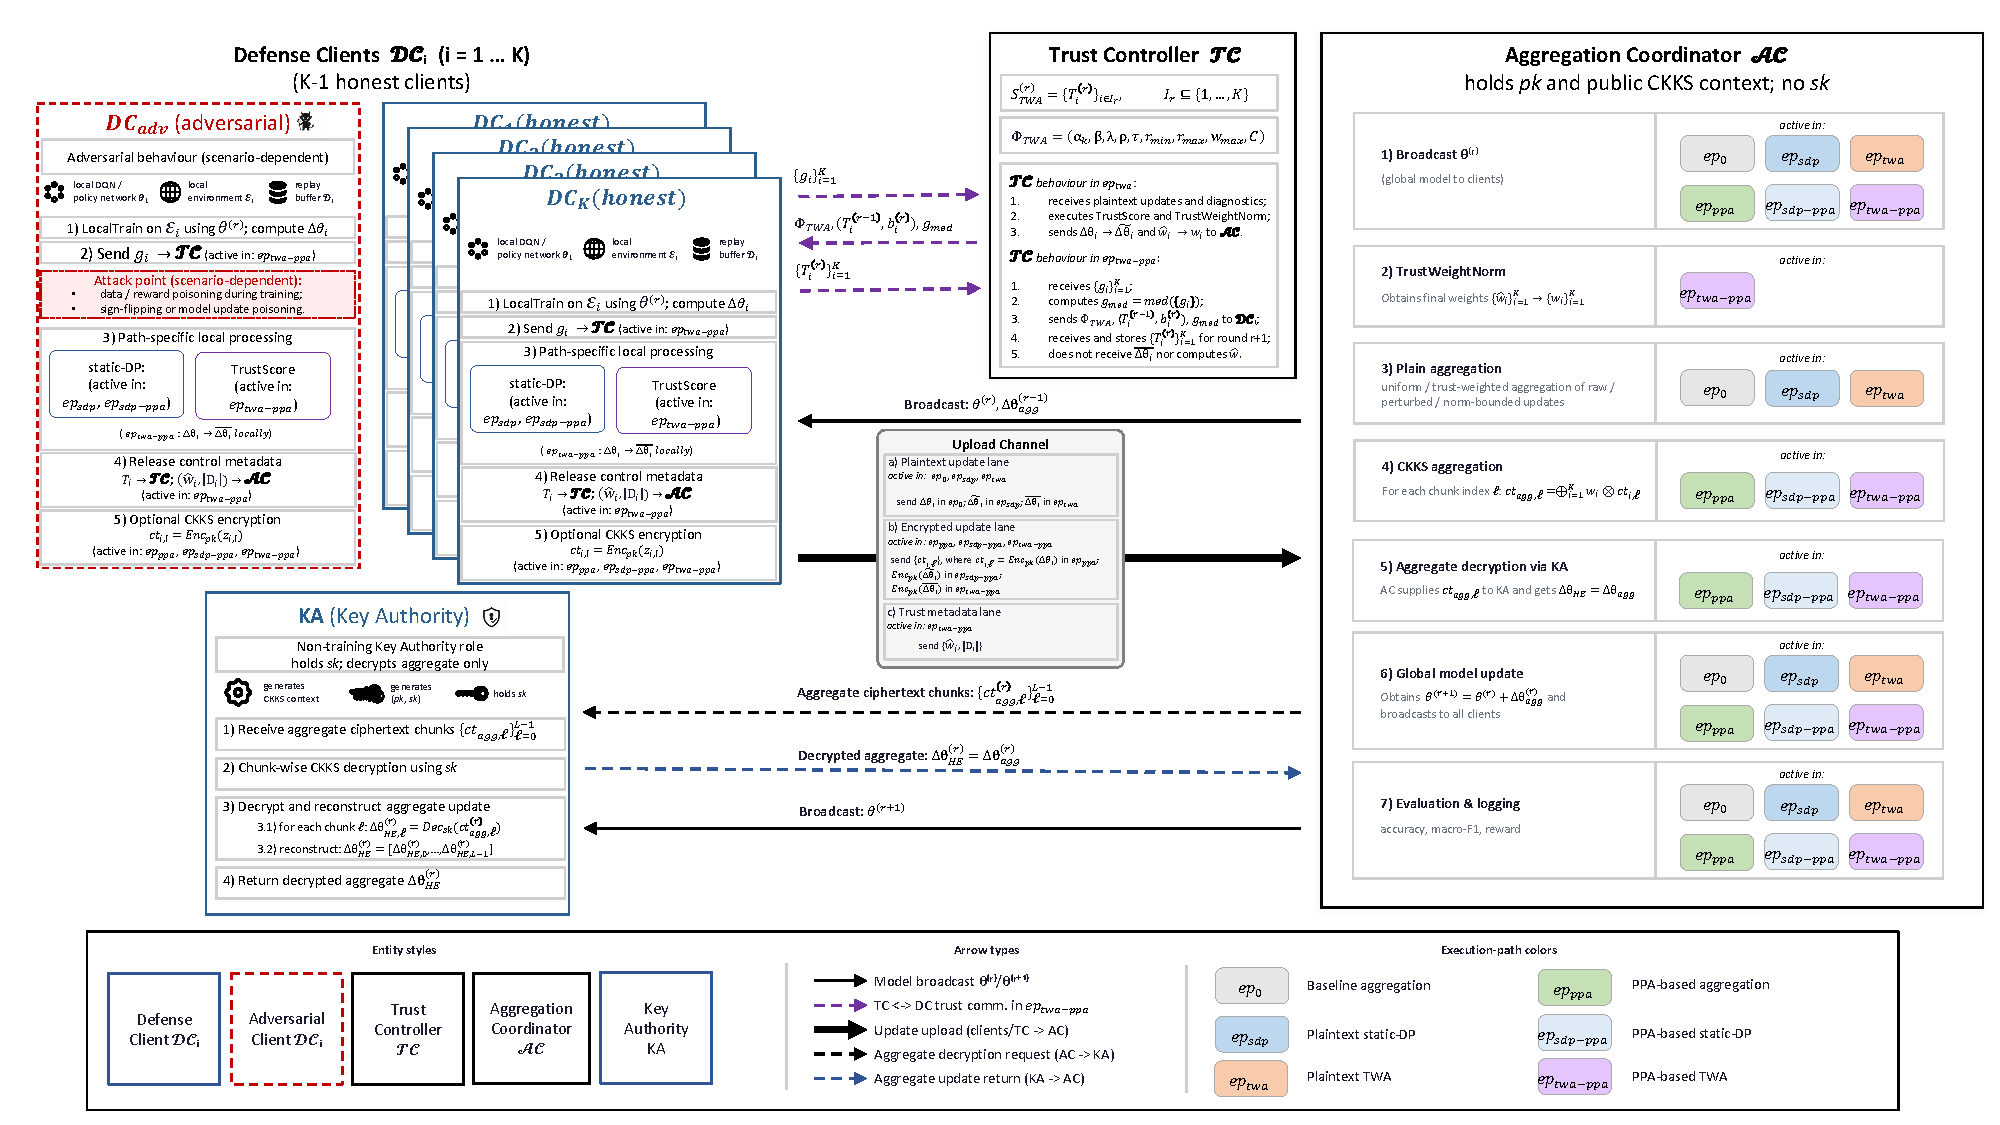
\includegraphics[width=\textwidth]{figures/system_architecture.pdf}
  \caption{Path-dependent FRL architecture with detailed TWA-PPA message flow.}
  \label{fig:system-overview}
\end{figure*}

\begin{itemize}

  \item \textbf{Defense Client ($\mathcal{DC}$):}
  Each $\mathcal{DC}_i$ maintains a local DQN model $\theta_i$, private
  environment $\mathcal{E}_i$, and replay buffer $\mathcal{D}_i$, and produces
  a round update $\Delta\theta_i^{(r)}$. In
  $ep_{\mathrm{twa\text{-}ppa}}$, it also executes the trust-scoring routine locally
  and encrypts the norm-bounded update.

  \item \textbf{Aggregation Coordinator ($\mathcal{AC}$):}
  $\mathcal{AC}$ maintains the global model, receives client update payloads,
  computes aggregation weights, and performs plaintext or homomorphic aggregation. 
  In encrypted paths, it holds $pk$ and the public CKKS context $pp$, but not $sk$.

  \item \textbf{Trust Controller ($\mathcal{TC}$):}
  $\mathcal{TC}$ manages the TWA policy and cross-round trust state. In
  $ep_{\mathrm{twa\text{-}ppa}}$, it computes $g_{\mathrm{med}}$ and
  distributes the inputs required for local trust scoring. In
  $ep_{\mathrm{twa}}$, trust scoring and normalization may instead execute
  centrally at $\mathcal{TC}$.

  \item \textbf{Key Authority ($\mathcal{KA}$):}
  $\mathcal{KA}$ generates the CKKS key pair, retains $sk$, and decrypts only
  aggregate ciphertexts received from $\mathcal{AC}$.

\end{itemize}

\subsection{Security Assumptions and Threat Model}

The proposed framework has path-dependent security objectives. We consider the
following entities and adversaries:

\begin{itemize}

  \item \textbf{Aggregation Coordinator ($\mathcal{AC}$).}
  $\mathcal{AC}$ is honest-but-curious and is assumed to follow the prescribed protocol. 
  In $ep_{\mathrm{twa\text{-}ppa}}$, it observes ciphertext update payloads, 
  the client trust metadata designated for $\mathcal{AC}$, and the 
  aggregation weights. It does not possess $sk$.

  \item \textbf{Defense Clients ($\mathcal{DC}$).}
  Clients may poison local data, rewards, or submitted updates as defined in
  Section~\ref{sec:exp_setup}. In the evaluated
  $ep_{\mathrm{twa\text{-}ppa}}$ setting, clients are assumed to execute
  \textsc{TrustScore} and report its metadata faithfully.

  \item \textbf{Trust Controller ($\mathcal{TC}$).}
  $\mathcal{TC}$ is assumed to follow the prescribed protocol.
  It may observe plaintext model updates in $ep_{\mathrm{twa}}$; in
  $ep_{\mathrm{twa\text{-}ppa}}$, it observes the client trust metadata
  designated for $\mathcal{TC}$ and the round diagnostic,
  but not current-round plaintext model updates.

  \item \textbf{Key Authority ($\mathcal{KA}$).}
  $\mathcal{KA}$ is trusted to retain $sk$ and decrypt aggregate ciphertexts
  only. Collusion with $\mathcal{AC}$ or access to individual client
  ciphertexts is outside the claimed model.

\end{itemize}

\noindent\textbf{Security objective.}
No update confidentiality is claimed for $ep_{0}$,
$ep_{\mathrm{sdp}}$, or $ep_{\mathrm{twa}}$. In
$ep_{\mathrm{ppa}}$, $ep_{\mathrm{sdp\text{-}ppa}}$, and
$ep_{\mathrm{twa\text{-}ppa}}$, individual updates remain encrypted during
aggregation, assuming that $sk$ remains with $\mathcal{KA}$ and only aggregate
ciphertexts are submitted for decryption. The permissible leakage
$\mathcal{L}$ is defined in Table~\ref{tab:notation}. 
The security proof for privacy-preserving aggregation paths is
given in Section~\ref{sec:security}.

\noindent\textbf{Information classes.}
We distinguish the public TWA policy
$\Phi_{\mathrm{TWA}}=\{\alpha_k,\beta,\lambda,\rho,\tau,r_{\min},r_{\max},w_{\max},C\}$,
cross-round trust state $\{T_i^{(r-1)}\}$, update-norm diagnostics
$\{g_i,g_{\mathrm{med}}\}$, released client trust metadata
$\{g_i,T_i,\hat{w}_i,|\mathcal{D}_i|\}$, aggregation weights $\{w_i\}$,
model-update payloads, public round state $(\theta^{(r)},
\Delta\theta_{\mathrm{agg}}^{(r-1)})$, and CKKS key material
$\mathcal{K}_{\mathrm{CKKS}}=\{pp,pk,sk\}$\footnote{
Descriptions of these classes and the destination-specific policy for releasing
client trust metadata are provided in Supplementary Section~2.1.}.
Their path-dependent flow is detailed in Section~\ref{sec:workflow_details}.

\subsection{Workflow Details}\label{sec:workflow_details}

We treat $ep_{\mathrm{twa\text{-}ppa}}$ as the main execution
path of the proposed framework. It consists of three client-side routines
(\textsc{LocalTrain}, \textsc{TrustScore}, \textsc{CKKSEncryptDelta}),
two aggregation-coordinator routines (\textsc{TrustWeightNorm},
\textsc{HEWeightedAggregate}), and one key-authority routine
(\textsc{DecryptAggregate}). The detailed pseudocode for the main workflow
(\textsc{TWA-PPA Workflow}) and its routines is provided in the Supplementary
Material (Algorithms~S1--S7). This path is evaluated against the related
frameworks discussed in Section~\ref{sec:related_comparison}.
The remaining execution paths follow the component definitions in
Section~\ref{sec:execution_paths}.

In $ep_{\mathrm{twa\text{-}ppa}}$\footnote{In $ep_{\mathrm{twa}}$, \textsc{TrustScore} 
is executed centrally at $\mathcal{TC}$.}, each $\mathcal{DC}_i$ trains locally on
$\mathcal{E}_i$, computes the raw update $\Delta\theta_i^{(r)}$, norm-bounds it
as $\bar{\Delta\theta}_i^{(r)}$, and executes \textsc{TrustScore} (Algorithm~S3)
locally before encryption. After receiving the preliminary weights
$\{\hat{w}_i\}_{i=1}^{K}$ and replay sizes $\{|\mathcal{D}_i|\}_{i=1}^{K}$,
$\mathcal{AC}$ executes \textsc{TrustWeightNorm} (Algorithm~S4) to obtain the 
final aggregation weights $\{w_i\}_{i=1}^{K}$.
Each client then encrypts $\bar{\Delta\theta}_i^{(r)}$ as ciphertext chunks
$\{\mathsf{ct}_{i,\ell}^{(r)}\}_{\ell=0}^{L-1}$ and uploads them to $\mathcal{AC}$.
The coordinator then performs chunk-wise homomorphic weighted aggregation to
obtain $\{\mathsf{ct}_{\mathrm{agg},\ell}^{(r)}\}_{\ell=0}^{L-1}$ without
using $sk$ and forwards only the aggregate ciphertext chunks to $\mathcal{KA}$.
The key authority recovers $\Delta\theta_{\mathrm{HE}}^{(r)}$ and returns this
aggregate update to $\mathcal{AC}$ to update and redistribute the global model.

The detailed steps of the $ep_{\mathrm{twa\text{-}ppa}}$ path are as follows:

\begin{enumerate}

\item \textbf{Initialization.}
Before the first round, $\mathcal{KA}$ generates or loads the CKKS context and
key pair $(pk,sk)$ under the parameters chosen in
Section~\ref{sec:param_selection}. It publishes $pk$ and the public CKKS
context $pp$ to all $\mathcal{DC}_i$ and to $\mathcal{AC}$, while retaining $sk$
outside $\mathcal{AC}$. $\mathcal{TC}$ loads the TWA configuration, including
clipping norm $C$, trust-component coefficients $\{\alpha_k\}$, smoothing
factor $\beta$, gating threshold $\lambda$, exponent $\rho$, and weight cap $w_{\max}$.
Each $\mathcal{DC}_i$ initializes its local DQN network $\theta_i$,
environment $\mathcal{E}_i$, replay buffer $\mathcal{D}_i$, and receives the public
CKKS context $pp$ when an encrypted path is used. $\mathcal{AC}$ initializes the public
global model $\theta^{(0)}$ in plaintext and broadcasts it to all clients.

\item \textbf{Global model broadcast.}
At the start of round $r$, $\mathcal{AC}$ sends the current global model
$\theta^{(r)}$ to every $\mathcal{DC}_i$. Each client loads $\theta^{(r)}$
into its local network before training begins.

\item \textbf{Local training and delta computation.}
Each $\mathcal{DC}_i$ executes \textsc{LocalTrain} (Algorithm~S2)
independently. The procedure runs $E$ local episodes in $\mathcal{E}_i$,
updating $\theta_i$ via DQN with $\varepsilon$-greedy exploration and experience
replay from $\mathcal{D}_i$. After training, the client computes the raw model
update $\Delta\theta_i^{(r)}=\theta_i^{\mathrm{local}}-\theta^{(r)}$ and records the
mean episode reward $\bar{r}_i$ and mean training loss $\bar{\ell}_i$. The local
F1 diagnostic $F_i^{\mathrm{raw}}$ is taken from local validation metrics when
available and otherwise set to the neutral implementation default $0.5$; the
update-norm diagnostic is $g_i=\|\mathsf{flatten}(\Delta\theta_i^{(r)})\|_2$.\footnote{
Adversarial attack-injection points used in the evaluation are defined in
Supplementary Section~2.4.}

\item \textbf{TWA trust scoring.}
First, $\mathcal{TC}$ provides the public trust policy constants
$\{\alpha_k,\beta,\lambda,\rho,\tau,r_{\min},r_{\max},w_{\max},C\}$
and the state pair $(T_i^{(r-1)},b_i^{(r)})$, where $b_i^{(r)}$ indicates that
no prior trust is stored for client $i$. It does not collect
the current-round plaintext deltas $\{\Delta\theta_i^{(r)}\}_{i=1}^{K}$ in
$ep_{\mathrm{twa\text{-}ppa}}$. Each client releases $g_i$ to $\mathcal{TC}$;
$\mathcal{TC}$ computes $g_{\mathrm{med}}=\mathsf{median}(\{g_i\}_{i=1}^{K})$
and distributes $g_{\mathrm{med}}$ to all clients before local trust scoring.
Each $\mathcal{DC}_i$ executes \textsc{TrustScore} (Algorithm~S3) locally 
using its own update $\Delta\theta_i^{(r)}$, local diagnostics 
$(|\mathcal{D}_i|,\bar{r}_i,\bar{\ell}_i,F_i^{\mathrm{raw}})$, its local
five-entry mean-reward history, update-norm diagnostics
$(g_i,g_{\mathrm{med}})$, trust state $(T_i^{(r-1)},b_i^{(r)})$, and the
previous public aggregate $\Delta\theta_{\mathrm{agg}}^{(r-1)}$ as the 
similarity reference. This produces the norm-bounded update 
$\bar{\Delta\theta}_i^{(r)}$, current trust score $T_i^{(r)}$, and preliminary weight 
$\hat{w}_i$. The client retains $\bar{\Delta\theta}_i^{(r)}$ locally until 
encryption, sends $T_i^{(r)}$ to $\mathcal{TC}$, and releases 
$(\hat{w}_i^{(r)},|\mathcal{D}_i|)$ to $\mathcal{AC}$ for weight normalization.

\item \textbf{TWA weight normalization.}
After receiving $\{T_i^{(r)}\}_{i=1}^{K}$ directly from the clients,
$\mathcal{TC}$ stores them as the trust state used in round $r+1$.
Separately, $\mathcal{AC}$ receives
$\{(\hat{w}_i^{(r)},|\mathcal{D}_i|)\}_{i=1}^{K}$ and executes
\textsc{TrustWeightNorm} (Algorithm~S4) to obtain the final public
aggregation weights $\{w_i^{(r)}\}_{i=1}^{K}$. The norm-bounded updates
remain local until encryption. The released trust metadata
$(T_i^{(r)}, \hat{w}_i^{(r)}, |\mathcal{D}_i|, w_i^{(r)})$
are treated as part of permissible leakage $\mathcal{L}$.

\item \textbf{CKKS chunk encryption.}
Each $\mathcal{DC}_i$ executes \textsc{CKKSEncryptDelta}
(Algorithm~S5) on $\bar{\Delta\theta}_i$. The routine flattens
the norm-bounded update into $\mathbf{z}_i\in\mathbb{R}^{P}$, partitions it into
$L=14$ chunks of $m_{\mathrm{slot}}=4096$ slots, zero-pads the final chunk, and
encrypts each chunk under $pk$ as
$\mathsf{ct}_{i,\ell}=\mathrm{Enc}_{pk}(\mathbf{z}_{i,\ell})$.

\item \textbf{Homomorphic weighted aggregation and decryption.}
$\mathcal{AC}$ executes \textsc{HEWeightedAggregate} (Algorithm~S6) to perform weighted aggregation
over the received ciphertext chunks using weights $\{w_i\}$, producing
encrypted aggregate chunks
$\{\mathsf{ct}_{\mathrm{agg},\ell}\}_{\ell=0}^{L-1}$ without using $sk$.
For each chunk index $\ell$, the coordinator forms
$\mathsf{ct}_{\mathrm{agg},\ell}=\bigoplus_{i=1}^{K}w_i\otimes\mathsf{ct}_{i,\ell}$.
$\mathcal{AC}$ forwards only the encrypted aggregate chunks to $\mathcal{KA}$
and never forwards individual client ciphertexts. The key authority
$\mathcal{KA}$ then executes \textsc{DecryptAggregate} (Algorithm~S7) to
decrypt, concatenate, strip padding, and reconstruct
$\Delta\theta_{\mathrm{HE}}$ to obtain $\Delta\theta_{\mathrm{agg}}^{(r)} \leftarrow
\Delta\theta_{\mathrm{HE}}$. $\mathcal{KA}$ returns this aggregate update to
$\mathcal{AC}$. This aggregate is in $\mathcal{L}$ because it is applied to
form the next public global model.

\item \textbf{Global model update, broadcast, and logging.}
After receiving $\Delta\theta_{\mathrm{HE}}$ from $\mathcal{KA}$, $\mathcal{AC}$
applies the recovered update $\Delta\theta_{\mathrm{agg}}^{(r)}$ to obtain
$\theta^{(r+1)}=\theta^{(r)}+\Delta\theta_{\mathrm{agg}}^{(r)}$, broadcasts the
updated model to all clients, and records accuracy, macro-F1, cumulative
reward, and path-specific diagnostics.
For TWA paths, $\mathcal{TC}$ records $\{T_i^{(r)}\}$,
while $\mathcal{AC}$ records $\{w_i^{(r)}\}$ and the resulting evaluation metrics.
This process repeats from step~2 until the configured number of rounds is 
completed or convergence is reached.

\end{enumerate}

\section{TRUST-WEIGHTED AGGREGATION}
\label{sec:trust_weighting}

\textbf{Trust model.}
Each client is assigned a trust score from six normalized indicators of
reward behavior, learning quality, update geometry, and trust history.
Specifically, $S_i$ denotes
reward stability, $Q_i$ the normalized local quality score, $M_i$ the
update--reference alignment component, $H_i$ the trust-history component,
$F_i$ the component derived from the local F1-score, and $G_i$ the
update-norm-deviation component.\footnote{Detailed component definitions are
provided in Supplementary Section~1.1; the complete scoring and normalization
routines and path-specific execution locations are provided in Supplementary
Section~1.2.}
Both TWA paths use the same scoring rule: $\mathcal{TC}$ evaluates it
centrally in $ep_{\mathrm{twa}}$, whereas each $\mathcal{DC}_i$ evaluates it
locally before encryption in $ep_{\mathrm{twa\text{-}ppa}}$.

The raw trust score is
\begin{equation}
\label{eq:trust}
T_{i,\mathrm{raw}} =
\alpha_S S_i +
\alpha_Q Q_i +
\alpha_M M_i +
\alpha_H H_i +
\alpha_F F_i +
\alpha_G G_i,
\end{equation}
where each component is normalized to $[0,1]$, the coefficients are
nonnegative, and
$\alpha_S+\alpha_Q+\alpha_M+\alpha_H+\alpha_F+\alpha_G=1$.
Across rounds, TWA maintains the smoothed trust estimate
\begin{equation}
\label{eq:trust_smooth}
T_i^{(r)} =
\begin{cases}
T_{i,\mathrm{raw}}^{(r)},
& \text{if client $i$ is first observed},\\[1mm]
\begin{aligned}
&\beta T_i^{(r-1)}\\[-1mm]
&\quad +(1-\beta)T_{i,\mathrm{raw}}^{(r)},
\end{aligned}
& \text{otherwise},
\end{cases}
\end{equation}
where $\beta\in[0,1]$ controls the contribution of previous trust.

\textbf{Trust-weighted aggregation.}
The smoothed trust score is converted into a preliminary aggregation weight
using the client's replay-memory size:
\begin{equation}
\label{eq:weights_prelim}
\hat w_i =
\begin{cases}
0, & T_i < \lambda,\\[1mm]
|\mathcal D_i|T_i^{\rho/\tau}, & T_i \geq \lambda,
\end{cases}
\end{equation}
where $\lambda$ is the low-trust suppression threshold, $\rho$ controls
trust-weight sharpening, and $\tau$ is its temperature parameter.
Algorithm~S4 converts these preliminary weights into final public aggregation
coefficients: it normalizes the positive mass, caps each client at
$w_{\max}$, and redistributes excess mass over the remaining eligible clients.
If all preliminary weights are zero, it falls back to replay-memory-size
weighting. Supplementary Section~1.2 gives the exact support updates,
feasibility condition, and redistribution procedure. The resulting weights
satisfy
\begin{equation}
\label{eq:weights}
0\leq w_i\leq w_{\max},
\qquad
\sum_{i=1}^{K}w_i=1.
\end{equation}
Thus, $\lambda$ controls explicit low-trust suppression, while $w_{\max}$
limits any one client's influence. TWA instantiates $a_i=w_i$ in
Eq.~\eqref{eq:global_update}; it changes the client-specific aggregation
coefficients rather than the global-update rule. In
$ep_{\mathrm{twa\text{-}ppa}}$, the same public coefficients multiply the
encrypted norm-bounded updates as described in
Section~\ref{sec:ppa_aggregation}. The reported numerical settings appear in
Section~\ref{sec:exp_setup}.

\section{PRIVACY-PRESERVING AGGREGATION}\label{sec:ppa_aggregation}

\textbf{CKKS configuration and model-update packing.}\label{sec:param_selection}
The CKKS parameters are selected to satisfy three requirements:
\emph{(C1)} at least 128-bit RLWE security,
\emph{(C2)} sufficient modulus depth for the ciphertext--plaintext weighted
aggregation circuit, and
\emph{(C3)} adequate numerical precision after aggregate reconstruction.
We use
\[
N=8192,
\qquad
\mathbf{q}=[60,30,60]\ \text{bits},
\qquad
\Delta=2^{30}.
\]
The resulting $150$-bit coefficient-modulus budget remains below the
$218$-bit limit recommended for $N=8192$ at the targeted security
level~\cite{albrecht2021he}. The circuit contains one
ciphertext--plaintext multiplication layer followed by ciphertext additions,
which is supported by the selected modulus chain. The chosen scale provides
sufficient precision for this depth-1 computation, as evaluated empirically in
Section~\ref{sec:experiments}.

Each client flattens its model update into
$\mathbf{z}_i\in\mathbb{R}^{P}$, where $P=53{,}636$. Since CKKS provides
$N/2=4096$ slots per ciphertext, the update is partitioned into
\[
L=\left\lceil\frac{P}{4096}\right\rceil=14
\]
contiguous chunks
$\mathbf{z}_{i,\ell}\in\mathbb{R}^{4096}$.
The first 13 chunks are fully occupied, while the final chunk contains
388 update values and 3708 zero-padding values. Each chunk is encrypted
independently:
\[
\mathsf{ct}_{i,\ell}
=
\mathrm{Enc}_{pk}(\mathbf{z}_{i,\ell}),
\qquad
\ell=0,\ldots,L-1.
\]

\textbf{Execution-path instantiation and TWA--PPA composition.}
\label{sec:twa_ppa_integration}
Let $\mu_i^{(r)}$ denote the configured non-robust baseline coefficient.
The six execution paths instantiate Eq.~\eqref{eq:global_update} as
\begin{equation}\label{eq:path_mapping}
(a_i^{(r)},u_i^{(r)})
=
\begin{cases}
(\mu_i^{(r)},\Delta\theta_i^{(r)}),
& ep_0,\;ep_{\mathrm{ppa}},\\
(\mu_i^{(r)},\widetilde{\Delta\theta}_i^{(r)}),
& ep_{\mathrm{sdp}},\;ep_{\mathrm{sdp\text{-}ppa}},\\
(w_i^{(r)},\bar{\Delta\theta}_i^{(r)}),
& ep_{\mathrm{twa}},\;ep_{\mathrm{twa\text{-}ppa}}.
\end{cases}
\end{equation}

In $ep_{\mathrm{twa\text{-}ppa}}$, TWA determines the aggregation operands
$(w_i^{(r)},\bar{\Delta\theta}_i^{(r)})$ before encryption, while PPA evaluates
the same linear aggregation rule over CKKS ciphertext chunks:
\begin{equation}\label{eq:he_agg}
\mathsf{ct}_{\mathrm{agg},\ell}^{(r)}
=
\bigoplus_{i=1}^{K}
w_i^{(r)}\otimes\mathsf{ct}_{i,\ell}^{(r)}.
\end{equation}
The weights $w_i^{(r)}$ are public plaintext scalars. After aggregate-only
decryption and reconstruction by $\mathcal{KA}$, the recovered
$\Delta\theta_{\mathrm{agg}}^{(r)}$ is applied through
Eq.~\eqref{eq:global_update} exactly as in the plaintext TWA path.
Thus, PPA changes the representation and execution of the aggregation, but not
its mathematical semantics. Trust scoring remains local, and the associated
metadata and aggregate output are treated as permissible leakage
$\mathcal{L}$.

\section{SECURITY ANALYSIS}\label{sec:security}

We now analyze the path-dependent security objective defined in
Section~\ref{sec:proposed_system} for the encrypted paths ($ep_{\mathrm{ppa}}$,
$ep_{\mathrm{sdp\text{-}ppa}}$, $ep_{\mathrm{twa\text{-}ppa}}$),
and we provide a proof sketch by reduction to the IND-CPA security of
CKKS~\cite{cheon2017ckks}, implemented with TenSEAL~\cite{benaissa2021tenseal},
under the RLWE assumption~\cite{peikertlattice2014}.

$\mathcal{AC}$ forwards only encrypted aggregate chunks
$\{\mathsf{ct}_{\mathrm{agg},\ell}\}$ to $\mathcal{KA}$, never individual
client ciphertexts $\mathsf{ct}_{i,\ell}$. If $\mathcal{KA}$ received
individual client ciphertexts, it could decrypt them with $sk$ and observe
the corresponding plaintext updates. If $\mathcal{AC}$ were itself
granted $sk$, or if $\mathcal{AC}$ and $\mathcal{KA}$ colluded to expose
individual ciphertexts, the individual-update confidentiality claim would no
longer apply.

\emph{Construction.}
In each round $r$, client $i$ flattens its local model delta
$\Delta\theta_i \in \mathbb{R}^P$ into $L = 14$ plaintext
chunks $\mathbf{z}_{i,\ell} \in \mathbb{R}^{m_{\mathrm{slot}}}$ with
$m_{\mathrm{slot}} = 4096$ slots and zero-padding on the last chunk.
Each chunk is encrypted under the shared public key $pk$ as
$\mathsf{ct}_{i,\ell} = \mathrm{Enc}_{pk}(\mathbf{z}_{i,\ell}) \in R_q \times R_q$,
where $R_q = \mathbb{Z}_q[X]/(X^N+1)$.
The CKKS ciphertext takes the form~\cite{cheon2017ckks}
$\mathsf{ct}_{i,\ell}
= \bigl(pk_0 \cdot u + e_0 + \lfloor \Delta \cdot \mathbf{z}_{i,\ell} \rceil,\;
pk_1 \cdot u + e_1\bigr)$,
where $u \leftarrow R_q$ is uniformly random, $e_0, e_1 \leftarrow \chi$ are
small error polynomials, and $\Delta = 2^{30}$ is the global scale.
Since $\mathbf{z}_{i,\ell}$ is masked by the random term $u$ and the scaled
noise $e_0$, the ciphertext $\mathsf{ct}_{i,\ell}$ is computationally
indistinguishable from a uniformly random element of $R_q \times R_q$ to
any adversary running in time $\mathrm{poly}(\lambda)$ without $sk$.
The coordinator aggregates chunk-wise using homomorphic weighted addition
$\mathsf{ct}_{\mathrm{agg},\ell}
= \bigoplus_{i=1}^{K} w_i \otimes \mathsf{ct}_{i,\ell}$,
where $\otimes$ is ciphertext--plaintext scalar multiplication and $\oplus$
is ciphertext addition.

\emph{Indistinguishability argument.}
\emph{Game.} Consider an adversary $\mathcal{A}$ running in time
$\mathrm{poly}(\lambda)$ controlling the honest-but-curious coordinator.
$\mathcal{A}$ selects two clients $i, j \in \{1, \ldots, K\}$ with local
deltas encoded as chunk sequences $\{\mathbf{z}_{i,\ell}\}$ and
$\{\mathbf{z}_{j,\ell}\}$. A challenger $\mathcal{C}$ samples
$b \leftarrow \{0,1\}$ and, for each chunk $\ell$, computes
$\mathsf{ct}_{b,\ell} \gets \mathrm{Enc}_{pk}(\mathbf{z}_{b,\ell})$,
then evaluates the homomorphic aggregate using all clients' ciphertexts.
$\mathcal{C}$ provides the coordinator's view
$\mathrm{View}_{\mathcal{A}}
= \bigl\{\{\mathsf{ct}_{i,\ell}\}_{i,\ell},
\{\mathsf{ct}_{\mathrm{agg},\ell}\}_{\ell},
\{w_i\}, pp, \mathcal{L}\bigr\}$
to $\mathcal{A}$, which then outputs a bit $b'$ and wins if $b' = b$.

\emph{Reduction.} Since each $\mathsf{ct}_{b,\ell}$ is produced by the
IND-CPA-secure $\mathrm{Enc}_{pk}(\cdot)$ of CKKS, and
$\mathsf{ct}_{\mathrm{agg},\ell}$ is a deterministic homomorphic computation
over the ciphertexts and public scalars $w_i$, the distribution of
$\mathrm{View}_{\mathcal{A}}$ depends on $b$ only through
$\mathbf{z}_{b,\ell}$. Any $\mathcal{A}$ distinguishing
$\mathrm{View}_{\mathcal{A}}^{(i)}$ from $\mathrm{View}_{\mathcal{A}}^{(j)}$
with non-negligible advantage can be used to construct $\mathcal{A}'$ that
breaks the IND-CPA security of CKKS with the same advantage, contradicting the
$(N, q, \chi, \Delta)$-RLWE assumption.\footnote{Single-round ciphertext
confidentiality, the limited multi-round freshness claim, and the permissible
leakage and excluded collusion cases are specified in Supplementary
Section~2.2.} Hence,
$\left|\,\Pr[b' = b] - \tfrac{1}{2}\,\right| \le \mathrm{negl}(\lambda)$.

\noindent\textbf{Key ownership.}
In the intended encrypted protocol, the CKKS context and public key $pk$ are
published to all defense clients and to $\mathcal{AC}$, while the secret key
$sk$ is held by a fixed designated key authority $\mathcal{KA}$ outside
$\mathcal{AC}$. The indistinguishability statements above assume that
$\mathcal{AC}$ holds only $(pk,pp)$ and never observes $sk$.

\section{EXPERIMENTS AND ANALYSIS}\label{sec:experiments}
To validate the proposed framework, we organize the evaluation into three experiments.
First, we measure clean and adversarial utility across all six execution paths under 
the six standalone attacks and contextualize the framework's clean-accuracy deviation against
source-reported results for representative robust-FL defenses.
Second, we extend the adversarial evaluation to varying federation sizes and malicious-client
ratios to quantify the robustness of the proposed framework.
Finally, we isolate the privacy-preserving aggregation layer by measuring runtime and
communication overhead for the PPA-enabled execution paths.

\subsection{Experimental Setup}\label{sec:exp_setup}

\textbf{Implementation.}
All experiments are conducted on a system running Ubuntu 22.04 with an Intel(R)
Core(TM) i7-12700 CPU @ 2.10GHz, 32~GB of RAM, and an NVIDIA GeForce RTX 3060 GPU.
We implemented the framework in Python 3.10 with PyTorch 2.0~\cite{paszke2019pytorch} 
for deep learning, TenSEAL 0.4~\cite{benaissa2021tenseal} for CKKS homomorphic encryption,
and NumPy~\cite{harris2020numpy} for numerical computations.
All execution paths use the same client partition, model architecture, and
training schedule unless otherwise stated.

\textbf{Dataset and Model.}
We evaluate distributed intrusion detection on a four-class subset of
CIC-IDS2017~\cite{sharafaldin2018cicids2017,unb_cicids2017}. Each flow's 78
numeric features form the state; the four actions predict \texttt{BENIGN},
\texttt{DDoS}, \texttt{PortScan}, or \texttt{FTP-Patator}, covering benign traffic, 
denial-of-service traffic, scanning traffic, and brute-force attack traffic. The reward is
$+3$ for a correct decision and $-2$ otherwise. Five fixed non-i.i.d. client
partitions train a shared
$78\!\rightarrow\!256\!\rightarrow\!128\!\rightarrow\!4$ DQN. All five
participants are benign in the clean setting; the adversarial setting
designates the fifth participant as malicious. Preprocessing, partition, seed policy, 
and DQN training hyperparameters are detailed in Supplementary Section~2.5.

\textbf{Execution Paths and Baselines.}\label{sec:execution_paths}
The six execution paths form a $3\times2$ design that combines three
update/aggregation modes with either plaintext or
privacy-preserving aggregation. The plaintext paths are $ep_{0}$,
$ep_{\mathrm{sdp}}$, and $ep_{\mathrm{twa}}$, while their
PPA-enabled counterparts are $ep_{\mathrm{ppa}}$,
$ep_{\mathrm{sdp\text{-}ppa}}$, and
$ep_{\mathrm{twa\text{-}ppa}}$\footnote{Detailed path-specific update and weighting 
rules are provided in Supplementary Section~2.3.}.

\textbf{Federated and Adversarial Setup.}
All six execution paths use the same four-class non-i.i.d. CIC-IDS2017 setting.
The five-client evaluation uses 30 rounds, one local episode capped at
16 steps, and one auxiliary supervised epoch per round. Experiment~1 uses five
benign clients when clean and a $(4+1)$ benign/malicious split under attack.
In Experiment 2, we extend the evaluation to varying federation sizes (5-20 clients) 
and malicious-client (20-40\%) ratios. Following a factorial evaluation
layout~\cite{nist_two_way_anova}, each execution path and each attack condition in
$\mathcal{A}_{\mathrm{single}}$ is treated as a separate factor.\footnote{Supplementary 
Section~2.4 defines the theoretical combined-attack space $\mathcal{A}_{\mathrm{eval}}$ 
and provides the standalone attack definitions and injection points.}
The clean and adversarial evaluations use three fixed seeds per configuration.
Results are reported as mean $\pm$ standard deviation across those seeds.


\textbf{Robustness and Privacy Configuration.}
The $ep_{\mathrm{sdp}}$ paths apply unit-$\ell_2$ clipping plus coordinate-wise
Gaussian noise ($\sigma=0.1$). Without privacy accounting, they are perturbation
baselines, not calibrated $(\varepsilon,\delta)$-DP
mechanisms~\cite{dwork2006dp,abadi2016dpdl}. For
reproducibility, the six-component TWA protocol abstraction uses trust coefficients
$\alpha_S=0.18$, $\alpha_Q=0.20$,
$\alpha_M=0.18$, $\alpha_H=0.10$, $\alpha_F=0.16$, and
$\alpha_G=0.18$; smoothing coefficient $\beta=0.65$; trust-weight exponent
$\rho=4.0$, corresponding to $\tau=1.0$; per-client aggregation cap
$w_{\max}=0.25$; and clipping norm $C=1.0$. The controlled path and
adversarial evaluations underlying Experiments~1--2 use the low-trust threshold
$\lambda=10^{-8}$, whereas the saved PPA correctness and overhead runs in
Experiment~3 use $\lambda=0.50$. The PPA parameters follow
Section~\ref{sec:ppa_aggregation}.


\subsection{Results and Analysis}\label{sec:results}

\noindent\textbf{Experiment 1: Global Utility.}
Table~\ref{tab:attack_path_performance} reports the round-30 accuracy and
macro-F1\footnote{Round-30 reward and mean round time for the same conditions, paths,
and seeds are reported in Supplementary Table~S4.} for the
baseline paths $ep_{0}$ and $ep_{\mathrm{ppa}}$, the static perturbation paths
$ep_{\mathrm{sdp}}$ and $ep_{\mathrm{sdp\text{-}ppa}}$, and the trust-weighted paths 
$ep_{\mathrm{twa}}$ and $ep_{\mathrm{twa\text{-}ppa}}$ under the clean setting denoted
by $\varnothing$ and the six single poisoning attacks in $\mathcal{A}_{\mathrm{single}}$.
Figure~\ref{fig:accuracy_loss_comparison} contextualizes TWA-PPA's clean-accuracy
deviation against representative robust-FL defenses~\cite{zhang_fldetector_2022,
nguyen_flame_2022,cao2021fltrust,fung_limitations_2020} described in
Section~\ref{sec:related_work}. Each value uses the closest matching baseline;
plaintext TWA isolates the utility effect of adding PPA.
Horizontal lines show source-reported ranges, filled markers show representative
values, and the dashed line and hollow marker denote the approximate value
inferred from the cited study.

\begin{figure}[!htbp]
\centering
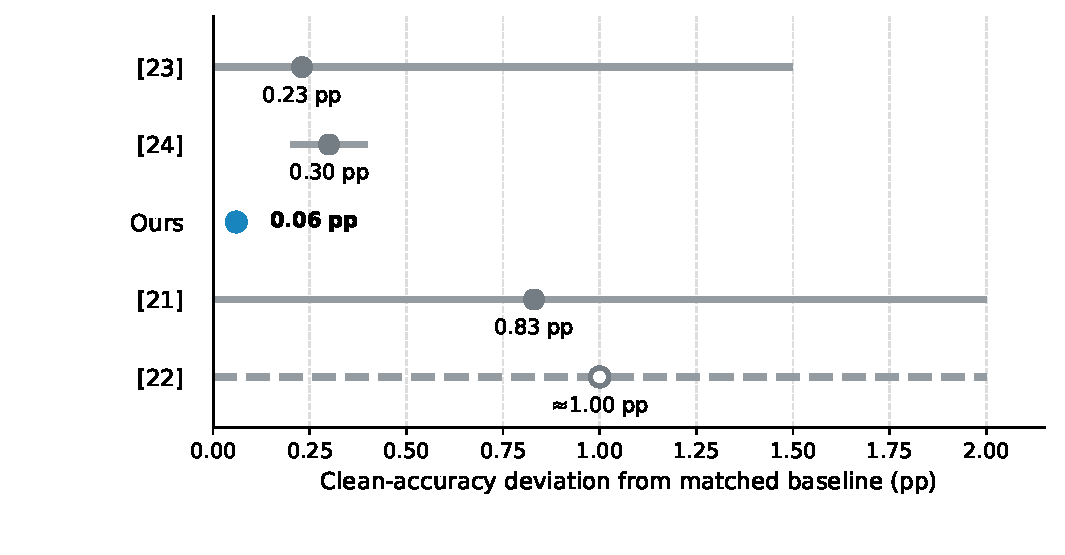
\includegraphics[width=\columnwidth]{figures/accuracy_loss_comparison.pdf}
\caption{Clean-accuracy deviation from each work's matched baseline. For
TWA-PPA, the marker is the mean paired absolute round-30 difference from
plaintext TWA across three fixed seeds ($0.06$ pp).}
\label{fig:accuracy_loss_comparison}
\end{figure}

\noindent\textbf{Experiment 2: Varying Federation Settings.}

Fig.~\ref{fig:sensitivity_scalability_summary} summarizes federation-size
sensitivity over three fixed seeds (mean $\pm$ standard deviation). Panel~(a) shows
accuracy (solid/filled) and macro-F1 (dashed/open); panel~(b) shows the malicious
clients' combined mean-round (solid/filled) and final-round (dashed/open)
weights; and panel~(c) shows the fraction of rounds at or below the $10^{-4}$
suppression cutoff. Supplementary Table~S3 reports the numerical results,
convergence gain, and round time.

\begin{table*}[!t]
\centering
\caption{Attack-Path Accuracy and Macro-F1 Across Three Fixed Seeds}
\label{tab:attack_path_performance}
\scriptsize
\setlength{\tabcolsep}{3pt}
\renewcommand{\arraystretch}{1.05}
\begin{tabular*}{\textwidth}{@{\extracolsep{\fill}}l c c c@{}}
\toprule
\multicolumn{4}{c}{\textbf{Panel A: Round-30 Accuracy / Macro-F1---non-encrypted paths}}\\
\midrule
Condition & $ep_0$ & $ep_{\mathrm{sdp}}$ & $ep_{\mathrm{twa}}$ \\
\midrule
$\varnothing$ & $0.5472\pm0.0588$ / $0.5055\pm0.0355$ & $0.4977\pm0.1164$ / $0.4208\pm0.1382$ & $0.9674\pm0.0037$ / $0.9668\pm0.0038$ \\
Sign flipping & $0.7077\pm0.1704$ / $0.6717\pm0.2011$ & $0.6006\pm0.0597$ / $0.5620\pm0.0673$ & $0.9707\pm0.0018$ / $0.9702\pm0.0018$ \\
RNB-Primary ($\alpha=0.5$) & $0.4369\pm0.1179$ / $0.3312\pm0.1424$ & $0.5647\pm0.2607$ / $0.5276\pm0.2961$ & $0.9708\pm0.0008$ / $0.9703\pm0.0008$ \\
Model replacement & $0.2093\pm0.0704$ / $0.0911\pm0.0154$ & $0.6409\pm0.0421$ / $0.5948\pm0.0755$ & $0.9737\pm0.0068$ / $0.9734\pm0.0068$ \\
Label flipping & $0.5992\pm0.1150$ / $0.5465\pm0.1700$ & $0.4636\pm0.0965$ / $0.3995\pm0.1081$ & $0.9712\pm0.0031$ / $0.9708\pm0.0032$ \\
Data poisoning & $0.5953\pm0.0671$ / $0.5774\pm0.0959$ & $0.5498\pm0.0956$ / $0.4745\pm0.1317$ & $0.9701\pm0.0008$ / $0.9696\pm0.0009$ \\
Reward poisoning & $0.5472\pm0.0588$ / $0.5055\pm0.0355$ & $0.4977\pm0.1164$ / $0.4208\pm0.1382$ & $0.9681\pm0.0027$ / $0.9675\pm0.0028$ \\
\bottomrule
\end{tabular*}

\vspace{1.2mm}

\begin{tabular*}{\textwidth}{@{\extracolsep{\fill}}l c c c@{}}
\toprule
\multicolumn{4}{c}{\textbf{Panel B: Round-30 Accuracy / Macro-F1---PPA-enabled paths}}\\
\midrule
Condition & $ep_{\mathrm{ppa}}$ & $ep_{\mathrm{sdp\text{-}ppa}}$ & $ep_{\mathrm{twa\text{-}ppa}}$ \\
\midrule
$\varnothing$ & $0.5512\pm0.0619$ / $0.5124\pm0.0445$ & $0.5000\pm0.1158$ / $0.4227\pm0.1375$ & $0.9678\pm0.0033$ / $0.9671\pm0.0034$ \\
Sign flipping & $0.7064\pm0.1593$ / $0.6718\pm0.1889$ & $0.5952\pm0.0583$ / $0.5541\pm0.0642$ & $0.9704\pm0.0017$ / $0.9700\pm0.0017$ \\
RNB-Primary ($\alpha=0.5$) & $0.4316\pm0.1176$ / $0.3251\pm0.1411$ & $0.5736\pm0.2749$ / $0.5348\pm0.3115$ & $0.9709\pm0.0010$ / $0.9704\pm0.0010$ \\
Model replacement & $0.2501\pm0.0002$ / $0.1021\pm0.0036$ & $0.6172\pm0.0843$ / $0.5717\pm0.1045$ & $0.9713\pm0.0043$ / $0.9710\pm0.0043$ \\
Label flipping & $0.5926\pm0.1359$ / $0.5458\pm0.1788$ & $0.4640\pm0.1057$ / $0.3957\pm0.1131$ & $0.9713\pm0.0035$ / $0.9709\pm0.0035$ \\
Data poisoning & $0.6379\pm0.1130$ / $0.6178\pm0.1360$ & $0.5433\pm0.0992$ / $0.4644\pm0.1411$ & $0.9698\pm0.0013$ / $0.9692\pm0.0014$ \\
Reward poisoning & $0.5496\pm0.0629$ / $0.5078\pm0.0408$ & $0.4951\pm0.1142$ / $0.4181\pm0.1361$ & $0.9682\pm0.0025$ / $0.9676\pm0.0026$ \\
\bottomrule
\end{tabular*}

\vspace{0.8mm}
\raggedright
\emph{Note:} Values are mean $\pm$ standard deviation across three fixed
seeds. Accuracy and macro-F1 are taken from round 30.
\end{table*}


\Needspace{15\baselineskip}
\noindent\textbf{Experiment 3: PPA Overhead.}

Figure~\ref{fig:roundwise_comm_overhead_combined} consists of two panels.
Panel~(a) reports only the source-scoped communication-expansion factors 
available for the representative works in Table~\ref{tab:comparison-related}; 
works without a compatible plaintext or FedAvg ratio are retained as N/A 
rather than assigned a value.
Panel~(b) retains source-reported absolute communication values with their
reported units and denominators: participant/iteration, participant/full-training,
and system/full-training values are green, blue, and orange, respectively.
These source-scoped values are not a normalized cross-paper benchmark.

\begin{figure}[H]
    \centering
    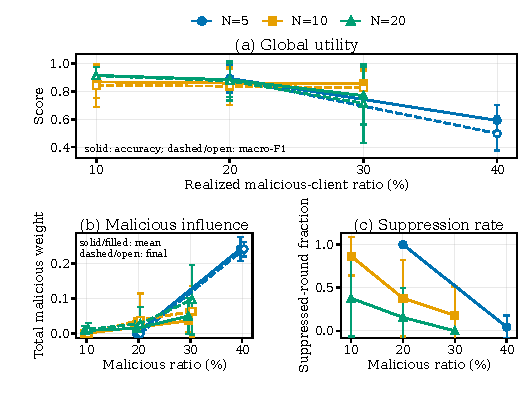
\includegraphics[width=\columnwidth]{figures/sensitivity_scalability_summary.pdf}
    \caption{TWA sensitivity across federation sizes and realized
    malicious-client ratios (mean $\pm$ SD over three fixed seeds).}
    \label{fig:sensitivity_scalability_summary}
\end{figure}

\noindent\textbf{Runtime Overhead.}
The corresponding runtime breakdown is summarized in Table~\ref{tab:runtime_overhead_table}
for six procedures (local training, preprocessing, encryption, aggregation, decryption, and evaluation)
and the total round time.

\begin{table}[H]
  \centering
  \caption{Runtime overhead by execution path.}
  \label{tab:runtime_overhead_table}
  \resizebox{\columnwidth}{!}{%
  \begin{tabular}{l c c c c c c c}
  \hline
  Path & LocalTrain & Preprocess & Encrypt & Aggregate & Decrypt & Eval & Round total \\
  \hline
  $ep_{0}$ & 9.319 & 0.000 & 0.000 & 0.003 & 0.000 & 0.525 & 9.849 \\
  $ep_{\mathrm{sdp}}$ & 9.025 & 0.002 & 0.000 & 0.002 & 0.000 & 0.515 & 9.546 \\
  $ep_{\mathrm{twa}}$ & 8.746 & 0.006 & 0.000 & 0.001 & 0.000 & 0.517 & 9.272 \\
  $ep_{\mathrm{ppa}}$ & 9.463 & 0.000 & 0.206 & 0.027 & 0.007 & 0.538 & 10.247 \\
  $ep_{\mathrm{sdp\text{-}ppa}}$ & 9.346 & 0.002 & 0.205 & 0.028 & 0.007 & 0.522 & 10.114 \\
  $ep_{\mathrm{twa\text{-}ppa}}$ & 8.989 & 0.006 & 0.207 & 0.070 & 0.007 & 0.524 & 9.807 \\
  \hline
  \end{tabular}}
\end{table}

\begin{table*}[!t]
\centering
\caption{Comparison With Representative Related Work}
\label{tab:comparison-related}
\footnotesize
\setlength{\tabcolsep}{2pt}
\renewcommand{\arraystretch}{0.92}
\resizebox{\textwidth}{!}{
\begin{tabular}{|c|c|c|c|c|c|c|c|c|c|}
\hline
\shortstack{\textbf{Work}} &
\shortstack{\textbf{Sys.}} &
\shortstack{\textbf{Priv./sec} \\ \textbf{agg.}} &
\shortstack{\textbf{Robust} \\ \textbf{agg.}} &
\shortstack{\textbf{Fed. attack} \\ \textbf{/ poisoning}} &
\shortstack{\textbf{Utility}\\\textbf{Loss}} & 
\shortstack{\textbf{Attack}\\\textbf{Results}} &
\shortstack{\textbf{Reported} \\ \textbf{comm. cost}} &
\shortstack{\textbf{Comp.} \\ \textbf{overhead}} &
\shortstack{\textbf{Storage}} \\
\hline

~\cite{bonawitz2017secagg} &
FL &
Masking &
N/A &
N/A &
N/A &
N/A &
\shortstack{$1.73{\times}$; $1.98{\times}$ clear/client\\
for selected source configurations} & 
\shortstack{C: $O(n^2+mn)$;\\ S: $O(mn^2)$} & 
\shortstack{C: $O(n+m)$;\\ S: $O(n^2+m)$} \\
\hline

~\cite{zhang2020batchcrypt} &
X-silo FL &
Paillier &
N/A &
N/A &
$<1\%$ &
N/A &
\shortstack{$1.60$--$2.50{\times}$ PT/\\
worker/iteration} &
\shortstack{23.3--92.8$\times$\\ speedup} & 
N/A \\
\hline

~\cite{manh2024homomorphic} &
FL-IoV &
CKKS &
N/A &
N/A &
$<0.8\%$ &
N/A &
N/A &
\shortstack{15--20 extra\\ iterations} &
N/A \\
\hline

~\cite{xuhercules2023} &
N-party FL &
MHE-CKKS &
N/A &
N/A &
$0.1$--$0.5$ pp &
N/A &
\shortstack{$0.59$--$17.58$ GB/user ($N{=}10$);\\
$474.61$--$8226.56$ GB/user ($N{=}50$),\\ FT} & 
\shortstack{$11.09$--$1540.43$ s ($N{=}10$);\\ $8.78$--$126.52$ h ($N{=}50$)} & 
\shortstack{$4.906$ GB (MNIST);\\ $16.47$ GB (CIFAR-10)} \\
\hline

~\cite{cao2021fltrust} &
FL &
N/A &
\shortstack{ReLU-cos;\\ norm; TWAvg} &
\shortstack{LF; Krum; Trim;\\ Sc.; Adap.} &
$\leq2$ pp & \shortstack{Acc. $90.4\%$;\\ ASR $1.3\%$} &
N/A & 
\shortstack{$O(np)$;\\ root update} & 
$O(|D_0|+np)$ \\
\hline

~\cite{fung_limitations_2020} &
FL &
N/A &
\shortstack{Cosine-sim.\\LR weighting} &
\shortstack{Sybil LF; Backdoor;\\ Perturb.; Adap.} &
N/A &
N/A &
N/A & 
\shortstack{$O(n^2d)$;\\ $<1.5$ s} & 
$O(nd)$ \\
\hline

~\cite{zhang_fldetector_2022} &
FL &
N/A &
\shortstack{Update-consist.\\client filtering} &
\shortstack{Untarg.; Sc.; DBA;\\ ALIE; Adap.} &
N/A &
\shortstack{Acc. $75.7\%$;\\ ASR $1.4\%$} &
N/A & 
$O(N^3+KBn^2+(6N+2n)p+Nn)$ & 
$O(Np)$ \\
\hline

~\cite{nguyen_flame_2022} &
FL &
N/A &
\shortstack{HDBSCAN;\\ clipping; DP-noise} &
\shortstack{C\&S; DBA; Edge-Case;\\ PGD; Untarg.; Adap.} &
$<0.4$ pp & \shortstack{Acc. $75.1\%$;\\ BA $1.3\%$} &
N/A &
\shortstack{$O(n^2p)$;\\ clustering} & 
$O(np+n^2)$ \\
\hline

~\cite{marx2026wwfl} &
Hier. FL &
MPC &
\shortstack{FLTrust; TM;\\ lightweight TM} &
\shortstack{RLF, TLF, SLF, DLF;\\ DaP only} &
\shortstack{MPC gap $<0.1\%$;\\ CIFAR-10 $+19.73$ pp} &
N/A &
\shortstack{$26.45$ TB/FT;\\ RA:\\
$9.69$ MB--$5.33$ GB} &
\shortstack{43.83 h;\\ $10{\times}$ faster} &
\shortstack{3.39 GB;\\ $250{\times}$ less} \\
\hline

~\cite{pillutla_robust_2022} &
FL &
SecAvg/MPC &
Geom. median &
\shortstack{Data poison;\\ Update poison;\\ Gaussian; Omniscient} &
$<1.4$ pp&
N/A &
\shortstack{$1$--$3{\times}$ FedAvg per RA} & 
$O(Rmd)$ &
N/A \\
\hline

\textbf{OURS} &
FRL-IDS &
CKKS &
Trust-weighting &
\shortstack{SF, RB, MR,\\ LF, DaP, ReP} &
\shortstack{TWA-PPA vs. TWA: no loss;\\
$0.06$ pp mean abs. dev.\textsuperscript{$\dagger$};\\
PPA: $0.40$ pp gain vs. $ep_0$} &
\shortstack{TWA-PPA mean\\ post-attack Acc.: $97.0\%$} &
\shortstack{$\approx13.4{\times}$ PT;\\
$2.745$ MiB/client/round;\\
$13.723$ MiB/round for $K{=}5$} &
\shortstack{Depth 1; $O(KL)$;\\ $9.807$ s/round} &
14 ct/client \\
\hline

\end{tabular}}

\vspace{0.8mm}
\raggedright
\emph{Note:} \textsuperscript{$\dagger$} Supplementary Table~S1 reports the
clean-utility calculation over three fixed seeds and the matched baseline. N/A~=~unreported;
C/S~=~client/server; Acc./BA/ASR~=~accuracy/backdoor accuracy/attack success rate;
PT/FT/RA~=~plaintext/full training/robust aggregation; TWAvg~=~trust-weighted averaging;
Sc./Adap./Untarg.~=~scaling/adaptive/untargeted attacks; and ct~=~ciphertext.
\end{table*}

\noindent\begin{minipage}{\columnwidth}
  \centering
  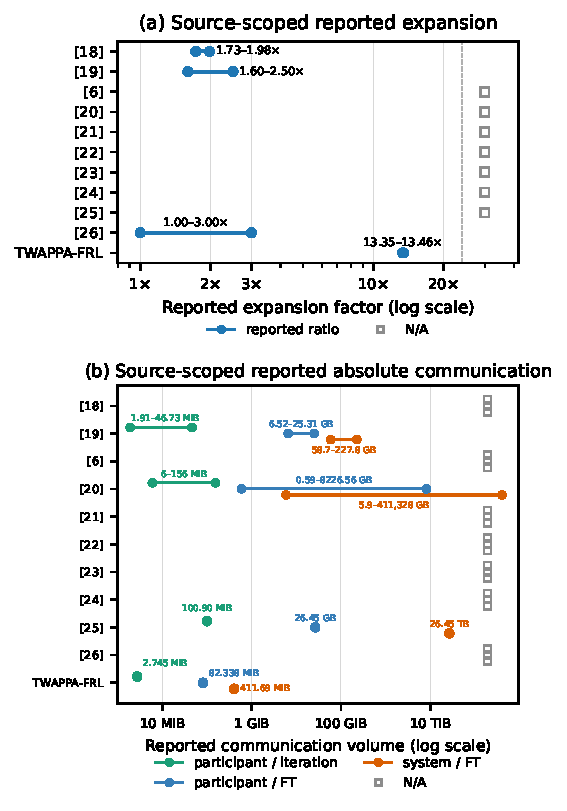
\includegraphics[width=0.92\columnwidth]{figures/roundwise_comm_overhead_combined_mb.pdf}
  \captionof{figure}{Source-scoped communication overhead.}
  \label{fig:roundwise_comm_overhead_combined}
\end{minipage}

\Needspace{6\baselineskip}
\noindent\textbf{Remark.} Accuracy is reported relative to each work's non-private, non-robust,
or plaintext baseline when available; otherwise, absolute values are used. Mean post-attack
accuracy summarizes adversarial performance.

\section{DISCUSSION}\label{sec:discussion}

\subsection{Future Work and Outlook}

Although the prototype validates joint trust-aware and confidential aggregation,
several directions remain. Future work should address \emph{(i)} broader
robustness evaluation across additional intrusion-detection datasets, larger
non-i.i.d. client populations, a broader set of fixed seeds, and adaptive or colluding
adversaries; \emph{(ii)} verifiable or attested trust computation to address
client-generated metadata forgery, which the current evaluation excludes;
\emph{(iii)} evaluation of lower-overhead confidential aggregation backends,
including quantized batching with additively homomorphic Paillier
encryption~\cite{zhang2020batchcrypt} and careful ciphertext layouts in multiparty
CKKS~\cite{xuhercules2023}, to substantially reduce HE communication and
computation overhead relative to the current CKKS path;
\emph{(iv)} removal of the fixed-key-authority assumption through threshold
FHE (ThFHE) decryption~\cite{dahl2023noahsark, hu2026ajax}, multiparty CKKS as used in
Hercules~\cite{xuhercules2023}, or secret-sharing-based MPC aggregation such
as SecretFlow-SPU~\cite{ma2023secretflowspu}, with their communication,
fault-tolerance, and non-collusion assumptions evaluated under realistic
network conditions; and \emph{(v)} quantification and reduction of leakage
through trust metadata, update norms, ciphertext sizes, and protocol timing
using secure computation, metadata coarsening, or controlled perturbation.

\subsection{Comparison With Related Work}\label{sec:related_comparison}

Table~\ref{tab:comparison-related} contrasts the proposed TWA-PPA framework
with representative federated learning systems discussed in
Section~\ref{sec:related_work}. Since the protected operation in this paper is
federated model-update release and aggregation, the comparison is organized
around: \emph{(i)} target system, \emph{(ii)} privacy-preserving or secure
aggregation mechanism, \emph{(iii)} robust aggregation mechanism,
\emph{(iv)} covered attack scenarios, including sign-flipping (SF), random
Byzantine behavior (RB), model-replacement/model-update poisoning (MR),
label-flipping (LF), data poisoning (DaP), and reward poisoning (ReP),
\emph{(v)} accuracy, \emph{(vi)} F1-score, \emph{(vii)} reward,
\emph{(viii)} adversarial-suppression metric, \emph{(ix)} communication volume,
\emph{(x)} computation complexity, and \emph{(xi)} storage overhead. Unreported
metrics are marked as not available rather than inferred.

\noindent\textbf{Remark.} The communication values in Table~\ref{tab:comparison-related}
retain source-native denominators and are not directly comparable across models,
federation sizes, training schedules, or protected operations.

\section{CONCLUSION}\label{sec:conclusion}

This paper presented TWAPPA-FRL, a path-dependent federated reinforcement
learning framework for privacy-preserving and trust-aware collaborative intrusion detection.
Across three fixed seeds in the five-client experiments with four benign and one malicious client,
the TWA-enabled paths achieved mean round-30 accuracy of
$0.9681$--$0.9737$ and macro-F1 of $0.9675$--$0.9734$ under six individual attacks.
At the $10^{-4}$ audit cutoff in the federation-sensitivity evaluation, the
suppressed-round fraction was $100\%$ with one malicious client among five and
$86.7\%$ with one among ten. In stress settings, it fell to $4.4\%$
with two malicious clients among five and zero with six among twenty; their combined
final weights nevertheless remained $0.240$ and $0.097$, below the corresponding
uniform shares of $0.40$ and $0.30$, demonstrating influence attenuation rather than exclusion.
The main TWA--PPA path matched plaintext TWA utility, required $9.807$~s per round
(dominated by local training), and uploaded $2.745$~MiB per client and
$13.723$~MiB system-wide per round. Together, these results position TWAPPA-FRL as a
confidential and trust-aware aggregation framework that retains detection utility
while shifting from threshold-level suppression to influence attenuation as malicious
participation increases.

\bibliographystyle{IEEEtran}
\bibliography{bibliography}

\newpage
\begin{IEEEbiography}[{
\includegraphics[width=1in,height=1.25in,clip,keepaspectratio]{figures/authors/piyumi.png}}]{PIYUMI M. S. RAJAPAKSHA}
~is currently pursuing the M.S. degree in the School of Cybersecurity and Information Law at the Chongqing University of Posts and Telecommunications.
Her research interests include federated learning, privacy-enhancing technologies, and cyber threat intelligence.
\end{IEEEbiography}

\begin{IEEEbiography}[{
\includegraphics[width=1in,height=1.25in,clip,keepaspectratio]{figures/authors/arturiasenovets.png}}]{ARTUR IASENOVETS}
~is currently pursuing the M.S. degree in the School of Cybersecurity and Information Law at the Chongqing University of Posts and Telecommunications.
His research interests include homomorphic encryption, systems for private search, retrieval, and processing of data.
\end{IEEEbiography}

\begin{IEEEbiography}[{
\includegraphics[width=1in,height=1.25in,clip,keepaspectratio]{figures/authors/YiyinXue.png}}]{YINXUE YI}
~received the M.E. and Ph.D. degrees from Chongqing University of Posts and Telecommunications, Chongqing, China,
in 2013 and 2021, respectively. She was with the Department of Computer Science, St. Francis Xavier University 
as a visiting student from February 2019 to March 2020. 
She is currently a Professor with the Chongqing University of Posts and Telecommunications, Chongqing, China. 
Her current main research interest includes social-physical networks, 
Internet of Things and information diffusion.
\end{IEEEbiography}

\begin{IEEEbiography}[{
\includegraphics[width=0.90in,height=1.25in,clip,keepaspectratio]{figures/authors/feitang.png}}]{FEI TANG}
~received the Ph.D. degree in information security from the Institute of Information Engineering,
Chinese Academy of Sciences, in 2015. He is currently a Professor with the Chongqing University of Posts and Telecommunications.
His research interests include public-key cryptography, data security, and so on.
\end{IEEEbiography}

\end{document}
